\sectionunnumbered{Appendix}

\begin{figure}[h]
    \centering
    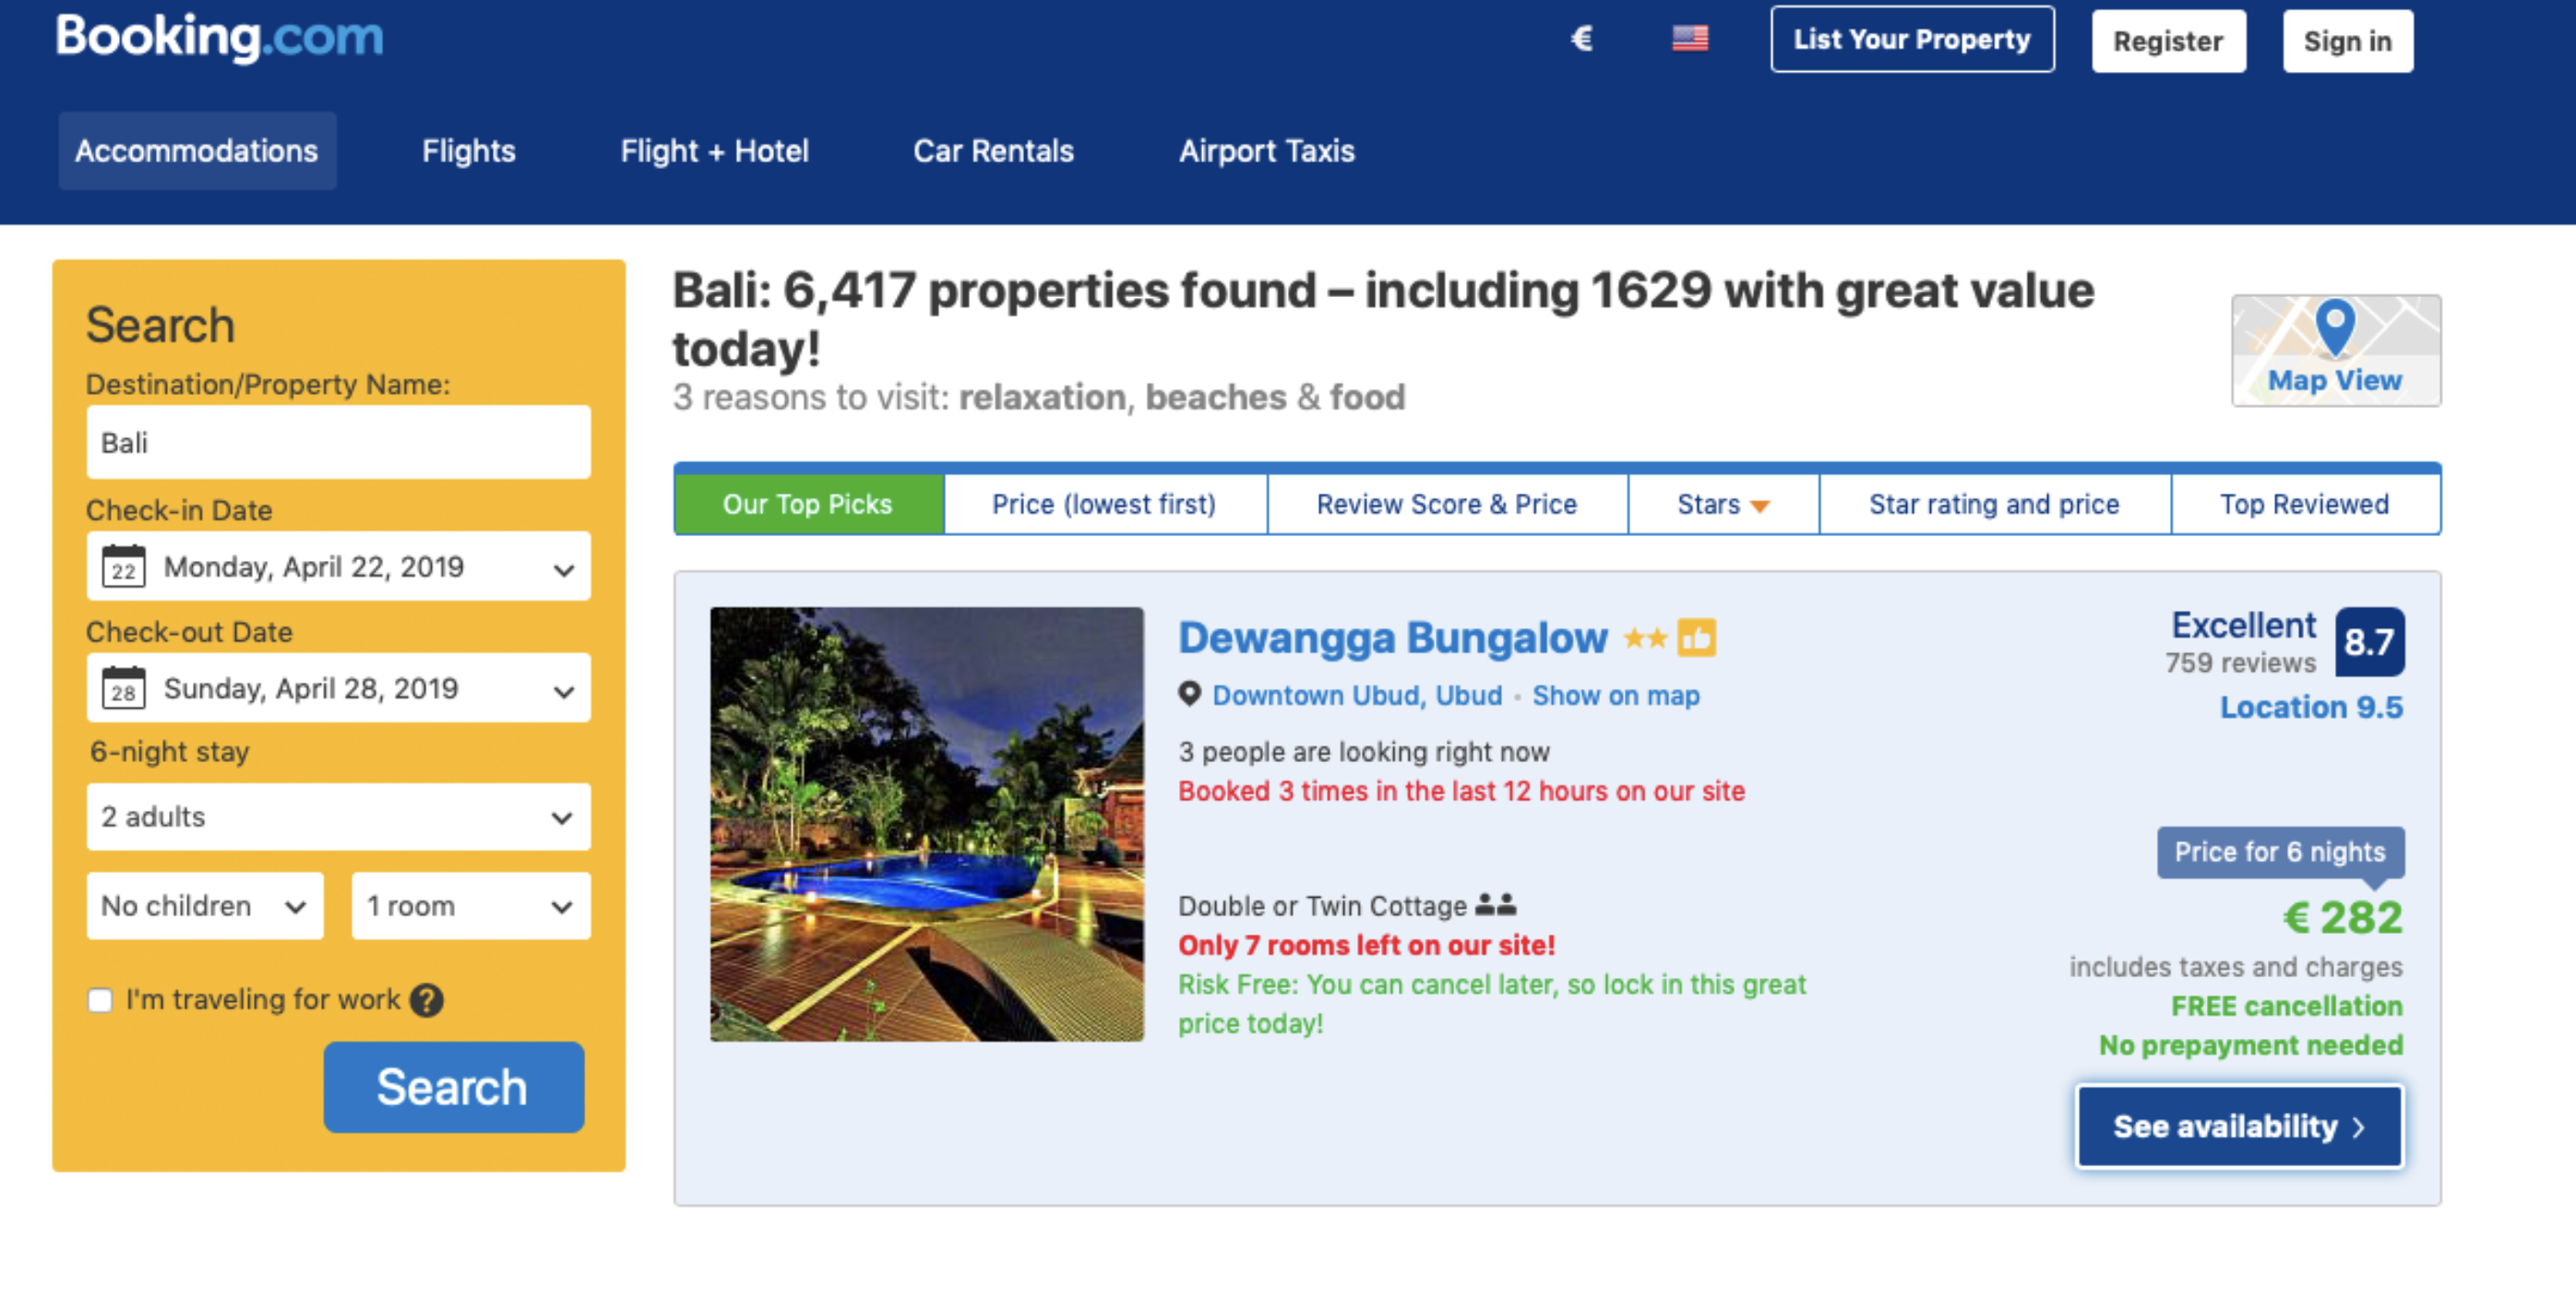
\includegraphics[width=1.0\textwidth]{booking-nudge.png}
    \caption{Digital nudging example - booking.com}
    \label{fig:booking}
\end{figure}

\newpage

\begin{table}[h!]
\begin{tabular}{|l|l|}
\hline
\textbf{Heuristic / Bias}  & \textbf{Example Design elements and mechanisms}                                                                                                                                                \\ \hline
Status quo bias            & \begin{tabular}[c]{@{}l@{}}- Radio buttons\\ - Checkboxes\\ - Dropdown menus\\ - Sliders with default position\\ - Pre-filled inputs\end{tabular}                                              \\ \hline
Decoy effect               & \begin{tabular}[c]{@{}l@{}}Presentation of options in: \\ - Radio buttons\\ - Checkboxes\\ - Dropdown menus\end{tabular}                                                                       \\ \hline
Primacy and recency effect & \begin{tabular}[c]{@{}l@{}}Positioning of elements \\ (earlier or later)\end{tabular}                                                                                                          \\ \hline
Middle-option bias         & \begin{tabular}[c]{@{}l@{}}- Addition of higher- and lower-price alternatives \\ around the preferred option.\\ - Ordering of alternatives.\\ - Modification of the option scale.\end{tabular} \\ \hline
Anchoring and adjustments  & \begin{tabular}[c]{@{}l@{}}- Variation of slider endpoints.\\ - Use of default slider position.\\ - Predefined values in text boxes for quantities.\end{tabular}                               \\ \hline
Norms (moral / social)     & \begin{tabular}[c]{@{}l@{}}- Display of popularity (social norms).\\ - Display of honesty codes (moral norms)\end{tabular}                                                                     \\ \hline
Scarcity effect            & \begin{tabular}[c]{@{}l@{}}- Use of default slider position.\\ - Language and displaying additional information \\ about quantity and availability \end{tabular} \\ \hline                               
\end{tabular}
\caption{Heuristics and Design elements of digital nudges (based on \cite{schneider_digital_2018})} 
\label{table:schneider}
\end{table}

\newpage


\begin{figure}[h]
    \centering
    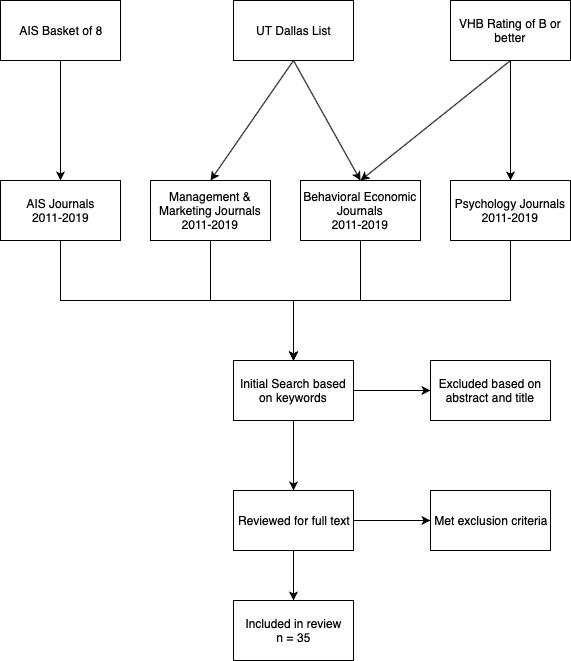
\includegraphics[width=1.0\textwidth]{method.png}
    \caption{Information flow of the screening process}
    \label{fig:method}
\end{figure}

\newpage

\begin{table}[h!]
\small
\centering
\begin{tabular}{|l|l|p{9cm}|l|}
\hline
 & \textbf{Library / Source} & \textbf{Journal} & \textbf{VHB Rating} \\ \hline
1 & AIS (Basket of 8) & European Journal of Information Systems & A \\ \hline
2 & AIS (Basket of 8) & Information Systems Journal & A \\ \hline
3 & AIS (Basket of 8) & Information Systems Research & A+ \\ \hline
4 & AIS (Basket of 8) & Journal of AIS & A \\ \hline
5 & AIS (Basket of 8) & Journal of Information Technology & A \\ \hline
6 & AIS (Basket of 8) & Journal of MIS & A \\ \hline
7 & AIS (Basket of 8) & Journal of Strategic Information systems & A \\ \hline
8 & AIS (Basket of 8) & MIS Quaterly & A+ \\ \hline
9 & UT Dallas & Journal on Computing & A \\ \hline
10 & UT Dallas & Journal of Consumer Research & A+ \\ \hline
11 & UT Dallas & Journal of Marketing & A+ \\ \hline
12 & UT Dallas & Journal of Marketing Research & A+ \\ \hline
13 & UT Dallas & Marketing Science & A+ \\ \hline
14 & UT Dallas & Management Science & A+ \\ \hline
15 & UT Dallas & Operations Research & A+ \\ \hline
16 & UT Dallas & Academy of Management Journal & A+ \\ \hline
17 & UT Dallas & Academy of Management Review & A+ \\ \hline
18 & UT Dallas & Journal of International Business Studies & A \\ \hline
19 & UT Dallas & Strategic Management Journal & A \\ \hline
20 & VHB & Journal of Behavioral Decision Making & B \\ \hline
21 & VHB & Journal of Behavioral and Experimental Economics & B \\ \hline
22 & VHB & Journal of Applied Behavioral Science & B \\ \hline
23 & VHB & Organizational Behavior and Human Decision Processes & A \\ \hline
24 & VHB & Applied Psychology & B \\ \hline
25 & VHB & European Journal of Work \& Organizational Psychology & B \\ \hline
26 & VHB & Journal of Applied Psychology & A \\ \hline
27 & VHB & Journal of Business and Psychology & B \\ \hline
28 & VHB & Journal of Consumer Psychology & A \\ \hline
29 & VHB & Journal of Economic Psychology & B \\ \hline
30 & VHB & Psychology \& Marketing & B \\ \hline
31 & AIS Conferences & Proceedings of the International Conference on Information Systems (ICIS) & A \\ \hline
32 & AIS Conferences & Proceedings of the European Conference on Information Systems (ECIS) & B \\ \hline
\end{tabular}
\caption{List of inspected journals}
\label{table:journals}
\end{table}

\newpage

\begin{figure}[h!]
    \centering
    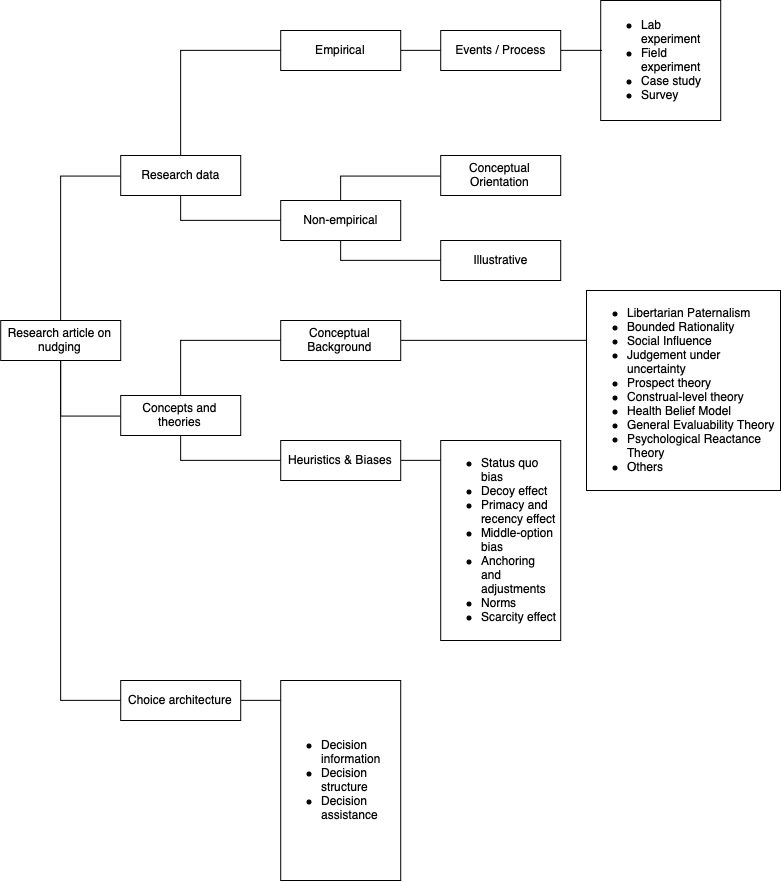
\includegraphics[width=1.0\textwidth]{analysis-2.png}
    \caption{Classification of findings-detailed}
    \label{fig:analysis-detail}
\end{figure}

\newpage

\begin{table}[h!]
\small
\begin{tabular}{|l|p{0.2\textwidth}|p{0.4\textwidth}|p{0.3\textwidth}|}
\hline
 & \textbf{Author \& Year} & \textbf{Title} & \textbf{Publication} \\ \hline
 1 & \cite{basu_choosing_2017} & Choosing one at a time? Presenting options simultaneously helps people make more optimal decisions than presenting options sequentially & Organizational Behavior and Human Decision Processes \\ \hline
2 & \cite{broniarczyk_decision_2014} & Decision Difficulty in the Age of Consumer Empowerment & Journal of Consumer Psychology \\ \hline
3 & \cite{bruns_can_2018} & Can Nudges Be Transparent and Yet Effective? & Journal of Economic Psychology \\ \hline
4 & \cite{cao_economic_2018} & An Economic Analysis of Peer Disclosure in Online Social Communities & Information Systems Research \\ \hline
5 & \cite{cosmo_nudging_2017} & Nudging electricity consumption using TOU pricing and feedback: evidence from Irish households & Journal of Economic Psychology \\ \hline
6 & \cite{dolan_influencing_2012} & Influencing behaviour: The mindspace way & Journal of Economic Psychology \\ \hline
7 & \cite{eigenbrod_how_2018} & How Digital Nudges Influence Consumers – Experimental Investigation in the Context of Retargeting & ECIS 2018 Proceedings \\ \hline
8 & \cite{faralla_framing_2017} & Framing effects in intertemporal choice: A nudge experiment & Journal of Behavioral and Experimental Economics \\ \hline
9 & \cite{gamliel_average_2017} & The Average Fuel-Efficiency Fallacy: Overestimation of Average Fuel Efficiency and How It Can Lead to Biased Decisions & Journal of Behavioral Decision Making \\ \hline
10 & \cite{goswami_when_2016} & When should the Ask be a Nudge? The Effect of Default Amounts on Charitable Donations & Journal of Marketing Research \\ \hline
11 & \cite{gravert_pride_2017} & Pride and patronage - pay-what-you-want pricing at a charitable bookstore & Journal of Behavioral and Experimental Economics \\ \hline
12 & \cite{guthrie_nudging_2015} & Nudging Consumers toward Better Food Choices: Policy Approaches to Changing Food Consumption Behaviors & Psychology \& Marketing \\ \hline
13 & \cite{hilton_tax_2014} & A tax can nudge: The impact of an environmentally motivated bonus/malus fiscal system on transport preferences & Journal of Economic Psychology \\ \hline
14 & \cite{huh_social_2014} & Social Defaults: Observed Choices Become Choice Defaults & Journal of Consumer Research \\ \hline
15 & \cite{hummel_designing_2017} & Designing Adaptibe Nudges for Multi-Channel Choices of Digital Services & ECIS 2017 Proceedings \\ \hline
\end{tabular}
\caption{List of reviewed research articles - Part 1}
\label{table:articles}
\end{table}

\newpage

\begin{table}[h!]
\small
\begin{tabular}{|l|p{0.2\textwidth}|p{0.4\textwidth}|p{0.3\textwidth}|}
\hline
 & \textbf{Author \& Year} & \textbf{Title} & \textbf{Publication} \\ \hline
16 & \cite{jones_effects_2015} & Effects of informational nudges on consumer debt repayment behaviors & Journal of Economic Psychology \\ \hline
17 & \cite{kretzer_designing_2018} & Designing Social Nudges for Enterprise Recommendation Agents: An Investigation in the Business Intelligence Systems Context & Journal of the Association for Information Systems \\ \hline
18 & \cite{lades_impulsive_2014} & Impulsive consumption and reflexive thought: Nudging ethical consumer behavior & Journal of Economic Psychology \\ \hline
19 & \cite{langley_should_2015} & Should I Get That Jab? Exploring Influence to Encourage Vaccination via Online Social Media & ECIS 2015 Proceedings \\ \hline
20 & \cite{laran_nonconscious_2018} & Nonconscious Nudges: Encouraging Sustained Goal Pursuit & Journal of Consumer Research \\ \hline
21 & \cite{lee_monochrome_2014} & Monochrome Forests and Colorful Trees: The Effect of Black-and-White versus Color Imagery on Construal Level & Journal of Consumer Research \\ \hline
22 & \cite{lembregts_making_2019} & Making Each Unit Count: The Role of Discretizing Units in Quantity Expressions & Journal of Consumer Research \\ \hline
23 & \cite{mazar_if_2018} & If You Are Going to Pay Within the Next 24 Hours, Press 1: Automatic Planning Prompt Reduces Credit Card Delinquency & Journal of Consumer Psychology \\ \hline
24 & \cite{miller_effects_2016} & The effects of pre-ordering and behavioral nudges on National School Lunch Program participants’ food item selection & Journal of Economic Psychology \\ \hline
25 & \cite{munscher_review_2016} & A Review and Taxonomy of Choice Architecture Techniques: Choice Architecture Techniques & Journal of Behavioral Decision Making \\ \hline
26 & \cite{romero_healthy-left_2016} & Healthy-Left, Unhealthy-Right: Can Displaying Healthy Items to the Left (versus Right) of Unhealthy Items Nudge Healthier Choices? & Journal of Consumer Research \\ \hline
27 & \cite{schneider_nudging_2017} & Nudging Users Into Online Verification: The Case of Carsharing Platforms & ICIS 2017 Proceedings \\ \hline
28 & \cite{sleesman_encouraging_2017} & Encouraging Prosocial Decisions: The Role of Fairness Salience and Uncertainty: Encouraging Prosocial Decisions & Journal of Behavioral Decision Making \\ \hline
\end{tabular}
\caption{List of reviewed research articles - Part 2}
\label{table:articles-2}
\end{table}

\newpage

\begin{table}[h!]
\small
\begin{tabular}{|l|p{0.2\textwidth}|p{0.4\textwidth}|p{0.3\textwidth}|}
\hline
 & \textbf{Author \& Year} & \textbf{Title} & \textbf{Publication} \\ \hline
29 & \cite{steffel_ethically_2016} & Ethically Deployed Defaults: Transparency and Consumer Protection through Disclosure and Preference Articulation & Journal of Marketing Research \\ \hline
30 & \cite{stryja_decision_2017} & A Decision Support System Design to Overcome Resistance Towards Sustainable Innovations & ECIS 2017 Proceedings \\ \hline
31 & \cite{szekely_nudging_2016} & Nudging People to Pay CO2 Offsets - The Effect of Anchors in Flight Booking Processes & ECIS 2016 Proceedings \\ \hline
32 & \cite{tietz_decoy_2016} & The Decoy Effect in Reward-Based Crowdfunding: Preliminary Results from an Online Experiment & ICIS 2016 Proceedings \\ \hline
33 & \cite{wang_socially_2018} & Socially Nudged: A Quasi-Experimental Study of Friends’ Social Influence in Online Product Ratings & Information Systems Research \\ \hline
34 & \cite{watson_swayed_2018} & Swayed by the Numbers: The Consequences of Displaying Product Review Attributes & Journal of Marketing \\ \hline
35 & \cite{yang_supremacy_2011} & The supremacy of singular subjectivity: Improving decision quality by removing objective specifications and direct comparisons & Journal of Consumer Psychology \\ \hline
36 & \cite{yoo_consumer_2018} & Consumer Choice and Market Outcomes Under Ambiguity in Product Quality & Marketing Science \\ \hline
37 & \cite{zarghamee_nudging_2017} & Nudging charitable giving: Three field experiments & Journal of Behavioral and Experimental Economics \\ \hline

\end{tabular}
\caption{List of reviewed research articles - Part 3}
\label{table:articles-3}
\end{table}

\newpage

\begin{table}[h!]
\centering
\begin{tabular}{|l|l|}
\hline
\textbf{Domain} & \textbf{Coding} \\ \hline 
Consumer Choice & CCH \\ \hline
Education & EDU \\ \hline
Finance & FIN \\ \hline
Health & HEA \\ \hline
Prosocial Behavior & PSB \\ \hline
Sustainability & SUS \\ \hline
Transportation & TRA \\ \hline
Security \& Privacy & SCP \\ \hline
Government & GOV \\ \hline
Other & MISC \\ \hline
\end{tabular}
\caption{List of domain codings}
\label{table:domain-coding}
\end{table}

\newpage

\begin{landscape}
\begin{table}
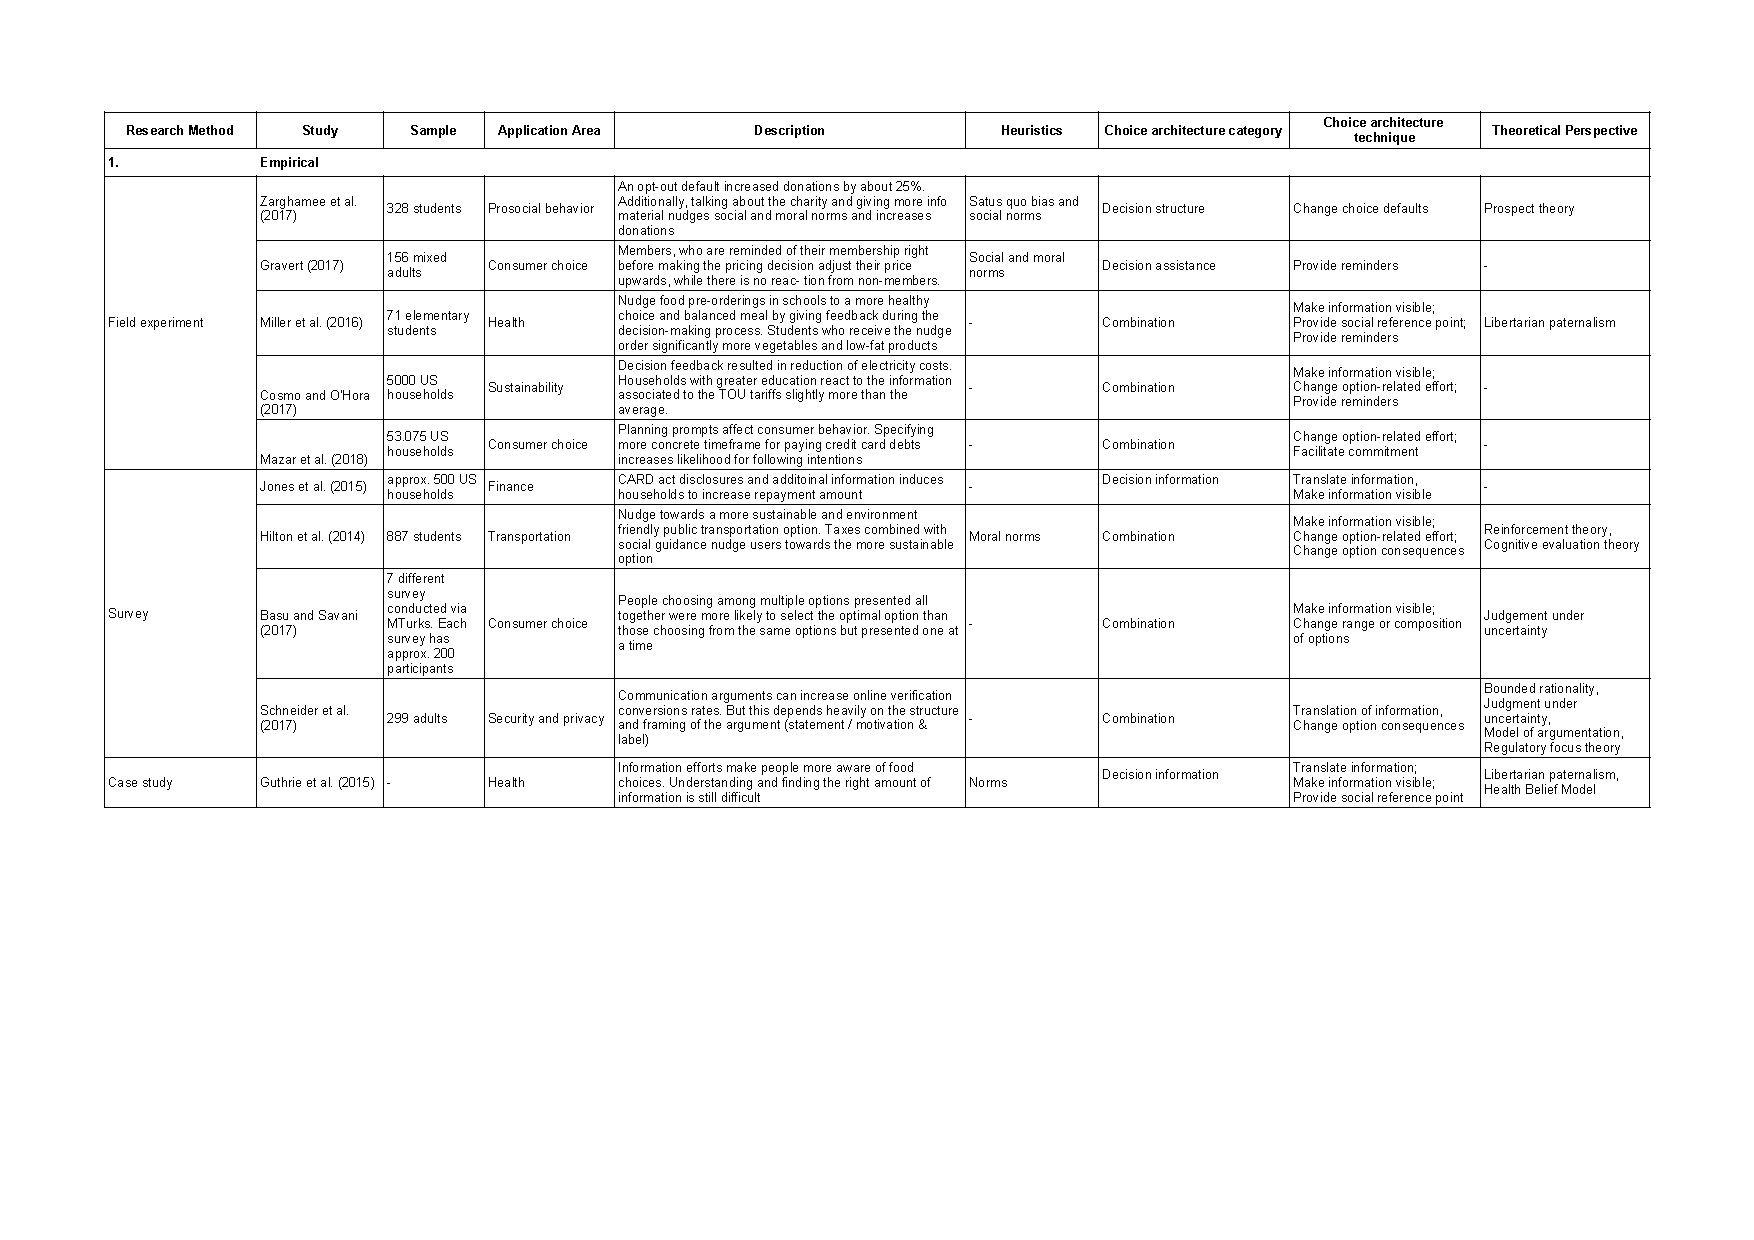
\includepdf[landscape=true, pagecommand={}]{coding.pdf}
\vspace{7cm}
\caption{Coding matrix of empirical studies}
\label{table:empirical-coding}
\end{table}
\end{landscape}

\newpage

\newpage

\begin{landscape}
\begin{table}
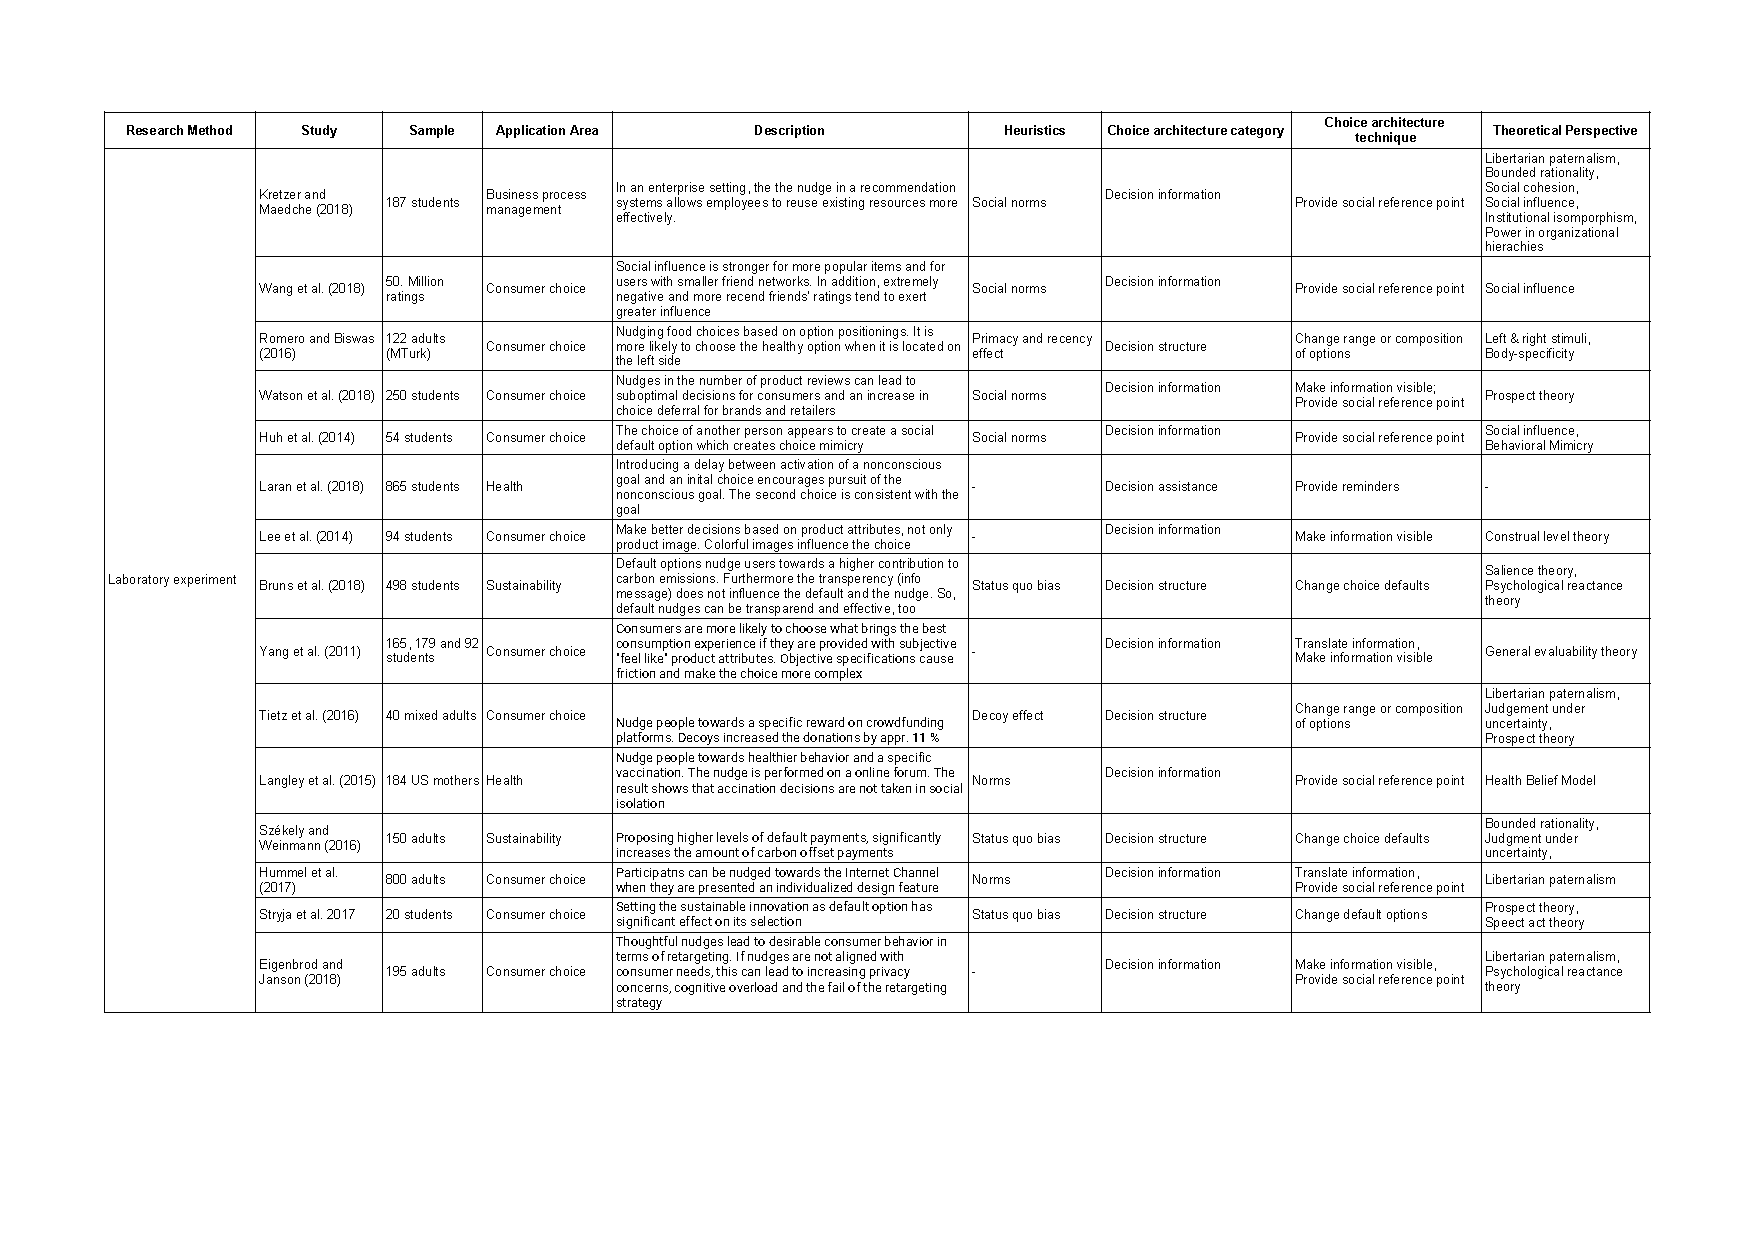
\includepdf[landscape=true, pagecommand={}]{coding-2.pdf}
\vspace{14cm}
\caption{Coding matrix of empirical studies - Part 2}
\label{table:empirical-coding-2}
\end{table}
\end{landscape}

\newpage


\newpage

\begin{landscape}
\begin{table}
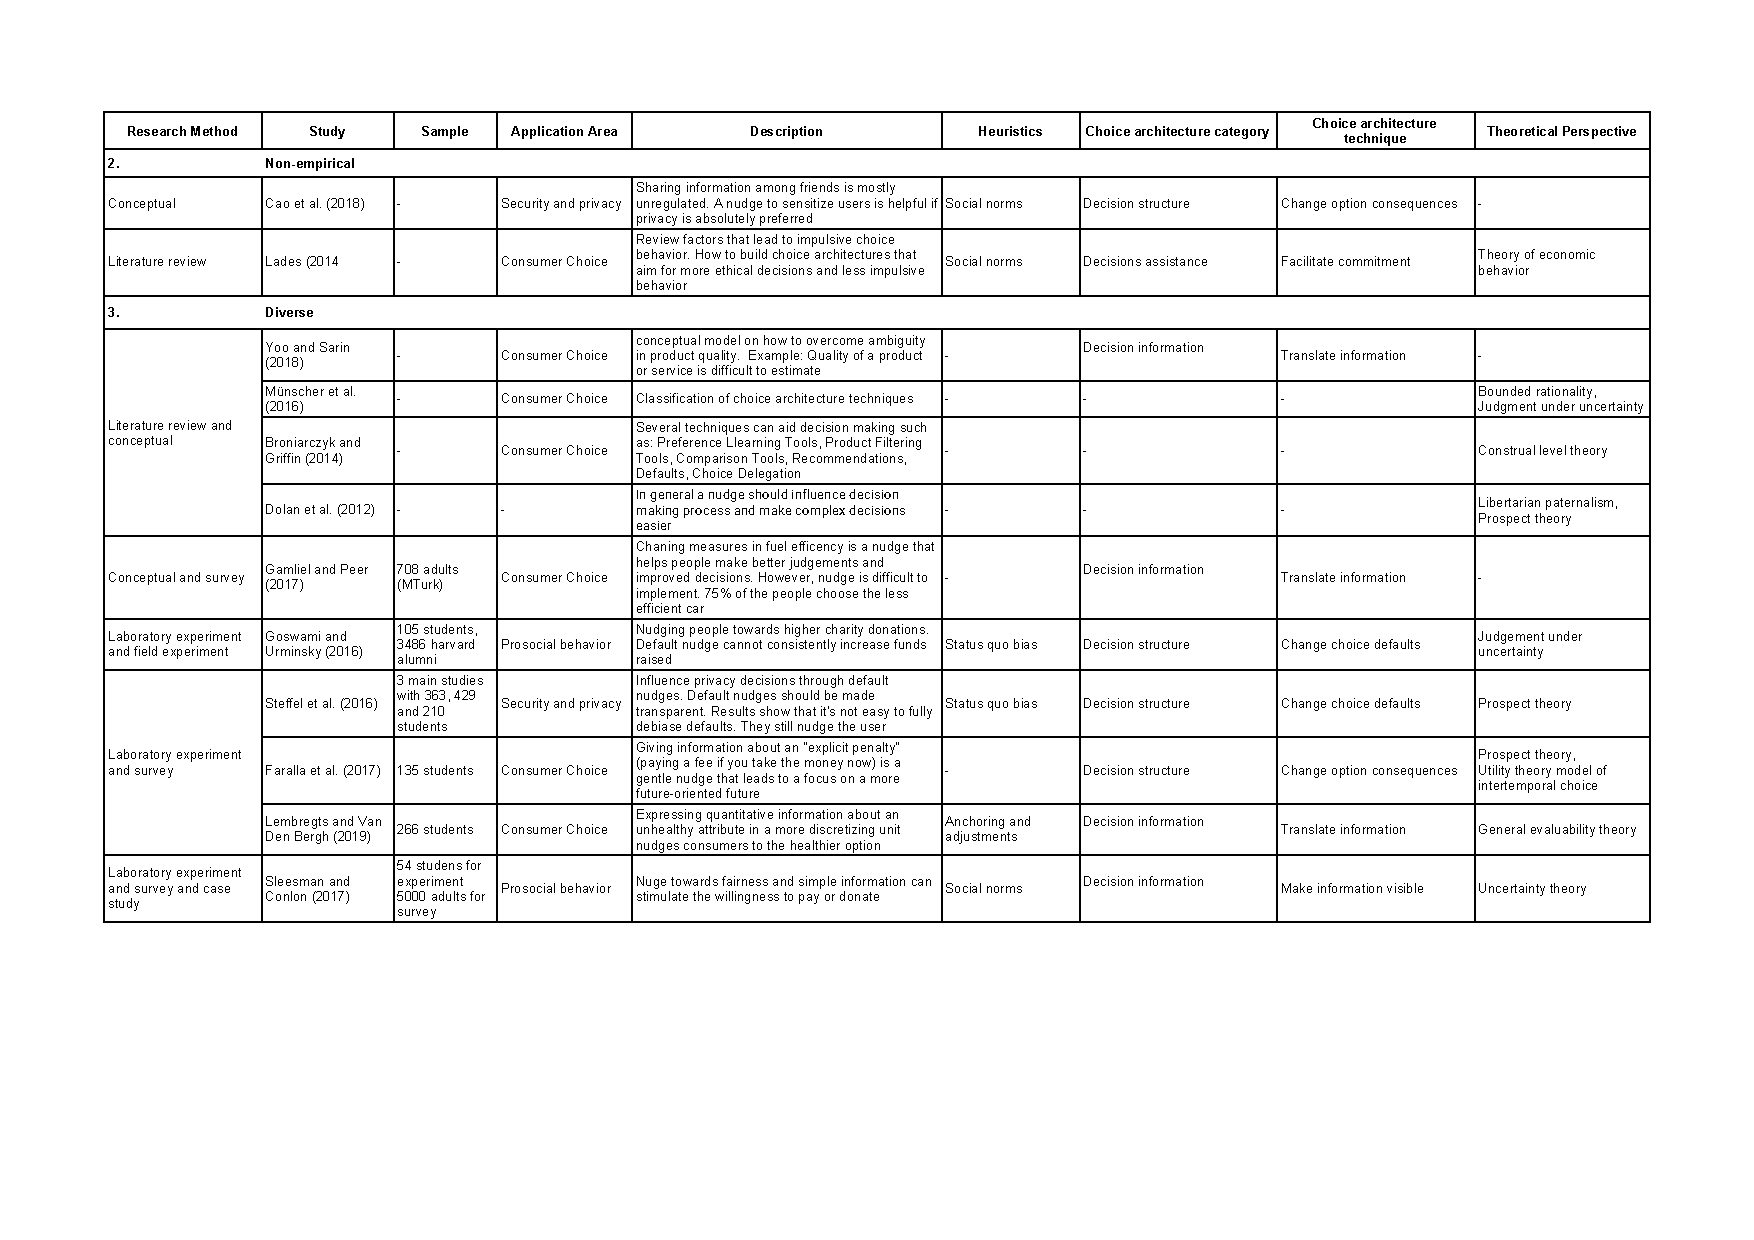
\includepdf[landscape=true, pagecommand={}]{coding-3.pdf}
\vspace{12cm}
\caption{Coding matrix of non-empirical and mixed studies}
\label{table:nonempirical-coding}
\end{table}
\end{landscape}

\newpage


\begin{table}[h!]
\small
\centering
\begin{tabular}{|p{0.2\textwidth}|p{0.8\textwidth}|}
\hline
\textbf{Coding category} & \textbf{Description} \\ \hline
Research method & Approach the researchers follow. This can be an empirical or non-empirical approach \\ \hline
Study & Reference to the author of the study and the year \\ \hline
Sample & Short summary of the sample of the study. Only if it follows an empirical approach \\ \hline
Application area & Based on the literature review, eight domains are identified. Consumer choice, education, finance, health, prosocial behavior, sustainability, transportation, security \& privacy, government. Additionally, other domains are summarized under the label "other" \\ \hline
Description & Summary of the study and the findings of the nudge experiment \\ \hline
Heuristics & Underlying cognitive heuristics and biases used to design the nudge \\ \hline
Choice architecture category & Based on Münscher et al. (\citeyear{munscher_review_2016}), three categories of choice architecture manipulations are used to classify the literature. Decision information, decision structure and decision assistance. If more than one category is changed, this is labeled is "combination" \\ \hline
Choice architecture technique & Based on the choice architecture categories, several techniques for a change are listed. The techniques are: translate information, make information visible, provide social reference points, change option-related effort, change range or composition of options, change option consequences, provide reminders and facilitate commitment \\ \hline
Theoretical perspective & If one ore more theoretical foundations are referenced in the study, they are listed here. \\ \hline
\end{tabular}
\caption{Description of coding categories}
\end{table}
